\paragraph{Two-strains Tuberculosis Model.}
Seeking to reduce the latent and infectious groups with the 
resistant-strain tuberculosis, in \cite{Lenhart2002} the authors  use 
controls ro represents 	two types of treatments in a tuberculosis model 
which consider the effect of treatment in two kinds of strains. The 
controlled version reads:
%
%	
%	\begin{equation}\label{eqn:two_strain_TB}
%	  \begin{aligned}
%	    \frac{dS}{dt} &=
%		    \Lambda - \beta_1 S \frac{I_1}{N} 
%		    - \beta_3 S \frac{I_2}{N}
%		    - \mu S
%		  \\
%		  \frac{L_1}{dt} &=
%			  \beta_1 S \frac{I_1}{N}
%			  - (\mu + k_1) L_1
%			  +  p r_2 I_1
%				+ \beta_2 T \frac{I_1}{N}
%				- \beta_3 L_1 \frac{I_2}{N}
%			\\
%			\frac{I_1}{dt} &= 
%				k_1 L_1
%				- (\mu + d_1) I_1
%				-r_2 I_1
%			\\
%			\frac{L_2}{dt} &=
%				q r_2 I_1
%				- (\mu + k_2) L_2
%				+ \beta_3 (S + L_1 + T) \frac{I_2}{N}
%			\\
%			\frac{I_2}{dt} &=
%				k_2 L_2 - (\mu + d_2) I_2
%			\\
%			\frac{d T}{dt} &=
%				r_1 L_1
%				+ (1 - (p + q)) r_2 I_1
%				- \beta T \frac{I_1}{N}
%				- \beta_3 T \frac{I_2}{N}
%				-\mu T ~.
%	  \end{aligned}
%	\end{equation}
%
%
	\begin{equation}\label{eqn:MDR-TB_model}
	  \begin{aligned}
	    \frac{dS}{dt} &=
		    \Lambda - \beta_1 S \frac{I_1}{N} 
		    - \beta_3 S \frac{I_2}{N}
		    \mu S
		  \\
		  \frac{L_1}{dt} &=
			  \beta_1 S \frac{I_1}{N}
			  - (\mu + k_1) L_1
			  - u_1 (t) r_1 L_1
			  + (1 - u_2 (t)) p r_2 I_1
				+ \beta_2 T \frac{I_1}{N}
				- \beta_3 L_1 \frac{I_2}{N}
			\\
			\frac{I_1}{dt} &= 
				k_1 L_1
				- (\mu + d_1) I_1
				-r_2 I_1
			\\
			\frac{L_2}{dt} &=
				(1 - u_2(t)) q r_2 I_1
				- (\mu + k_2) L_2
				+ \beta_3 (S + L_1 + T) \frac{I_2}{N}
			\\
			\frac{I_2}{dt} &=
				k_2 L_2 - (\mu + d_2) I_2
			\\
			\frac{d T}{dt} &=
				u_1(t) r_1 L_1
				+ (1 - (1 - u_2(t))(p + q)) r_2 I_1
				- \beta T \frac{I_1}{N}
				- \beta_3 T \frac{I_2}{N}
				-\mu T.
	  \end{aligned}
	\end{equation}

	\citeauthor*{Lenhart2002} consider time dependent 
optimal control strategies associated with \emph{case holding} and 
\emph{case finding}. They 
incorporates the case finding control by adding a term which identifies and 
cure a fraction o latent individuals. Case finding consequently reduces the 
rate of disease development by latent individuals. The authors includes case 
holding by adding a term which may decrease the treatment failure rate of 
individuals with sensitive  TB, so, this control reduce the incidence of drug 
resistant TB. In model \eqref{eqn:MDR-TB_model}, $u_1$ denotes the fraction of 
typical TB latent individuals that is identified and will put under 
treatment \textemdash case finding control \textemdash and $1 - u_2$ represents 
the effort that prevents the failure treatment in typical TB infectious 
individuals.

	The controls $u_1$ ,$u_2$ reduce the latent and infected 
groups with resistant TB. However, the case holding and the case finding 
strategies produces a economic fee. In \cite{Lenhart2002} the authors use
\begin{equation}
	 J(u_1, u_2) =
		 \int_0 ^ {t_f}
			 \left[
				 L_2(t) + I_2(t) 
				 + \frac{B_1}{2} [u_1(t)] ^ 2
				 + \frac{B_2}{2} [u_2(t)] ^ 2
			 \right]dt,
\end{equation}
to describe the regarding cost.
\begin{table}
	\centering
	\begin{tabular}{rll}
		\toprule
			& \multicolumn{1}{c}{\textbf{Description}} & \textbf{Simulation values}
            \\
        \midrule
        $\beta_1$ 
            & Probability that a susceptible 
            \\
            & individual becomes infected.
            & \num{13.0}            
            \\
        $\beta_2$ 
        	& Probability that a recovered 
        	\\
        	& individual  become infected
        	& \num{13.0}
        	\\
        $\beta_3$ 
        	& Probability that a uninfected 
        	\\
        	& individual become infected 
            & \num{0.0131}, 
              \num{0.0217},
            \\
            & by resistant-TB 
            & \num{0.029}, 
              \num{0.0436}
       		\\
     	\\
     	$\mu$ 
     	    & Natural per-capita death rate.
     	    & \num{0.0143}
			\\
     	$d_1$ 
     	    & Per-capita death rate by TB.
     	    & \num{0.0}
     	    \\
     	$d_2$ 
     	   	& Per-capita  death rate by MDR-TB.
     	   	& \num{0.0}
     	    \\
     	\\
     	$k_1$ 
     		& Rate at which an latent TB 
     		\\
     		& individual becomes infectious. 
     		& \num{0.5}
 			\\
     	    $k_2$  
     	    & Rate at which an latent individual
     	    \\
     	    & with MDR-TB becomes infectious.
     	    & \num{1.0}
		\\
		\\
		$r_1$ & 
      		Treatment recover rate of 
      		\\
      		& individuals with latent TB.
      		& \num{2.0}
     	    \\
		$r_2$ 
			& Treatment rate recover of 
			\\
			& individuals with infectious TB.
		
			& \num{1.0}
     	    \\
     	    $p$, $q$
     	    & Proportion of infectious individuals 
     	    \\
     	    & that not complete the treatment  
     	    & \num{0.4}, \num{0.1}
     	    \\
     	    & for TB or MDR-TB respectively
		\\
		\\	
			$N$ 
			& Total population size
			& 
			\num{6000}, 
			\num{12000}, 
			\num{30000}
            \\
			$\Lambda$ 
				& Recruitment rate
				& $\mu N$
            \\
            $t_f$ 
            & Final time 
            & \num{5.0} years
      \\
      \\
     	    $B_1$ 
     	    & Systematic cost of the 
     	    \\
     	    & case finding  control
     	    & \num{50.0}
			\\
     	    $B_2$
     	    & 
     	    Cost of the case holding strategy
     	    & \num{500.0}
     	    \\
     	    & Control lower bound  & $0.05$
			\\
            & Control upper bound & $0.95$
       		\\
       		\\
		&&\multicolumn{1}{c}{\textbf{Initial Conditions}}
		\\
		\cmidrule{3-3}
		&&	
		$S(0) = (76/120)N$
		\\
		&&
		$L_1(0) = (36/120) N$
		\\
		&&
		$I_1(0) = (4/120)N$
		\\
		&&
		$L_2(0) =(2/120) N$
		\\
		&&
		$I_2(0) = (1/120)N$
		\\
		&&
		$T(0)= (1/120)N$
		\\
		\bottomrule
    \end{tabular}
	\caption{Parameters description and simulation values for the control 
	problem \eqref{eqn:MDR-TB_model}.}
	\label{tbl:parameters_MDR-TB_model}
\end{table}


	In \cref{fig:figure1twostraintbm} we show the effect of case finding and 
case holding controls. The combination of this strategies diminish the multi 
drug resistant population. In \cref{tbl:parameters_MDR-TB_model} we compile the 
parameters description and values used to produce this figure and fix 
$N = \num{30000}$, $\beta_3 = \num{0.29}$. To minimize the resistant TB 
population, L2 + I2, the simulation suggest that the case holding strategy 
$u_2$ would be at the upper bound during almost \num{4.3} years and then 
decreasing to the lower bound. Meanwhile, decreasing value for case finding
must apply over the most of the simulated time, 5 years. The total number of 
infected resistant TB $L2 + I2$  at the final time $t_f = 5(years)$ results
\num{1123}. This same number but without control sums 4176. So this policies 
prevents  \num{3053} (= 4176 − 1123) cases of resistant TB.


\begin{figure}
  \centering
  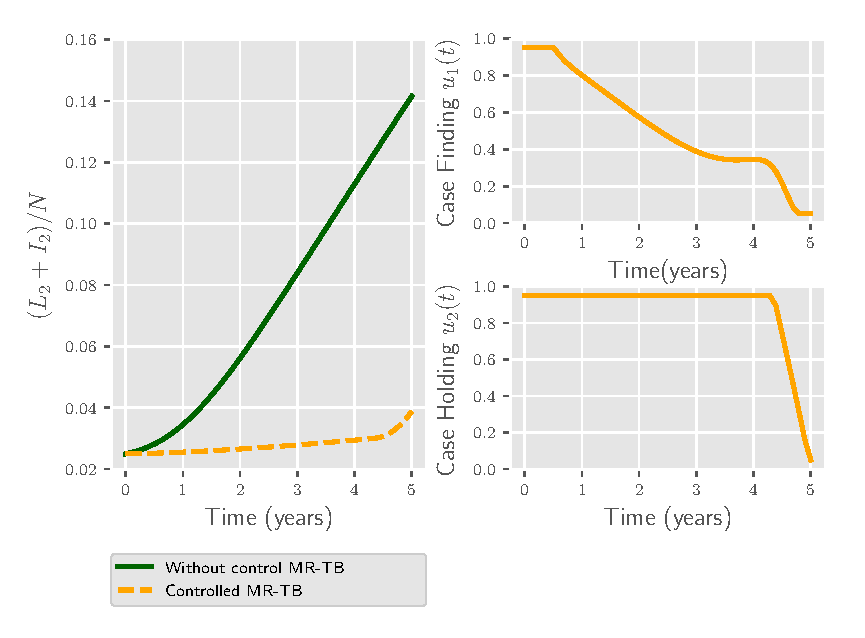
\includegraphics[width=0.7\linewidth]{Figures/figure_1_two_strain_tbm}
  \caption{Normalized infected population according to the parameters in 
  table [*]. Here the green line represents the infected population without 
  control. As we see, case finding $u_1(t)$ and case holding $u_2(t)$, 
  dramatically diminish the density of infected with resistant TB.}
  \label{fig:figure1twostraintbm}
\end{figure}


In figure [] we show the effect of the parameter $\beta_3$. As wee see the 
simulation suggest that...

\begin{figure}
  \centering
  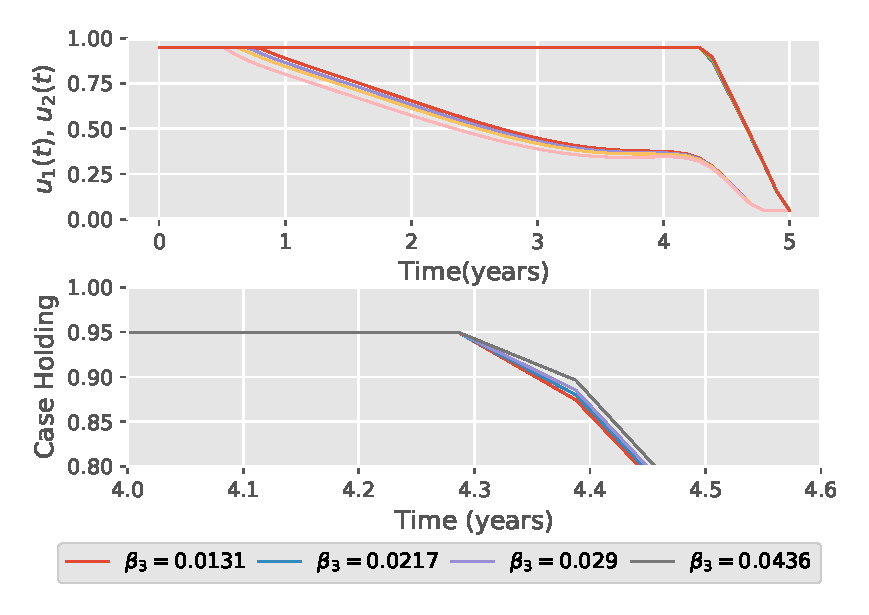
\includegraphics[width=0.7\linewidth]{Figures/figure_2_two_strain_tbm}
  \caption{}
  \label{fig:figure2twostraintbm}
\end{figure}

In figure we use different sizes of whole populations.
\begin{figure}
\centering
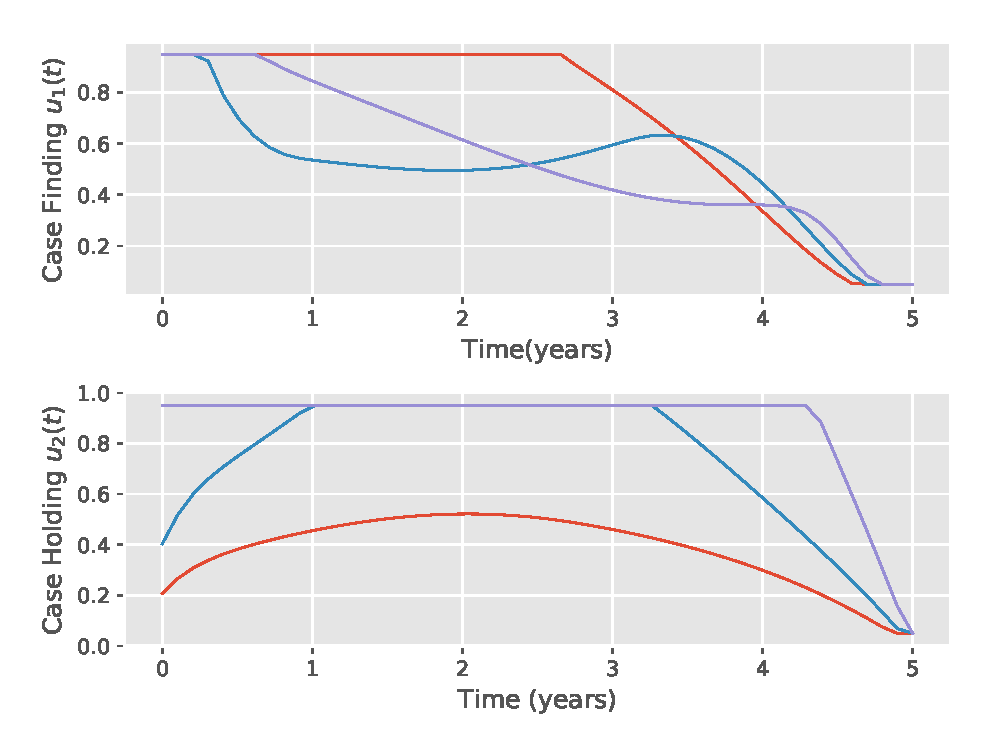
\includegraphics[width=0.7\linewidth]{Figures/figure_3_two_strain_tbm}
  \caption{The effect of different size of populations. As we see for 
  relatively small population, the case finding strategie is more importatn 
  than case finding, meanwhile for relateviley big populations the case holding 
  plays a more important role.}
  \label{fig:figure3twostraintbm}
\end{figure}



